\begingroup
\setlength{\abovedisplayskip}{6pt}
\setlength{\belowdisplayskip}{6pt}
\setlength{\abovedisplayshortskip}{4pt}
\setlength{\belowdisplayshortskip}{4pt}
\setlength{\intextsep}{6pt}

The given system has mass $m=12\ \mathrm{kg}$, stiffness $k=655\ \mathrm{N/m}$, damping coefficient $c=19\ \mathrm{N\,s/m}$, initial displacement $u_0=3.5\ \mathrm{mm}$, and initial velocity $\dot{u}_0=0$. Using $N_{\mathrm{osc}}=10$ sets the plotted interval to ten damped oscillations.

{ % do not increment counter
\begin{center}\small\begin{tabular}{@{}lrl@{}}
\toprule\noalign{}
Quantity & Value & Unit \\
\midrule\noalign{}
$m$ & 12.0 & kg \\
$k$ & 655 & N/m \\
$c$ & 19.0 & N s/m \\
$u_0$ & 3.50 & mm \\
$\dot{u}_0$ & 0 & mm/s \\
$N_{\mathrm{osc}}$ & 10 & -- \\
\bottomrule\end{tabular}\end{center}
}

The natural frequency follows from the stiffness-to-mass ratio. Converting it to hertz requires division by $2\pi$.

\[
\omega_n=\sqrt{\frac{k}{m}}=\sqrt{\frac{655}{12}}=7.388\ \mathrm{rad/s},
\qquad
f_n=\frac{\omega_n}{2\pi}=1.176\ \mathrm{Hz}.
\]

\[
\boxed{\omega_n=7.39\ \mathrm{rad/s},\qquad f_n=1.176\ \mathrm{Hz}}
\qquad\text{(B.3.2)}
\]

Critical damping is the value that makes the characteristic-equation discriminant equal to zero. Therefore,

\[
c_{\mathrm{cr}}=2\sqrt{mk}=2\sqrt{(12)(655)}=177.313\ \mathrm{N\,s/m}.
\]

\[
\boxed{c_{\mathrm{cr}}=177.3\ \mathrm{N\,s/m}}
\qquad\text{(B.3.3)}
\]

The damping ratio compares the actual damping with the critical value. Since $c<c_{\mathrm{cr}}$, the system is underdamped.

\[
\zeta=\frac{c}{c_{\mathrm{cr}}}=\frac{19}{177.313}=0.107155.
\]

\[
\boxed{\zeta=0.1072\quad\text{(underdamped)}}
\qquad\text{(B.3.4)}
\]

For an underdamped system, the oscillatory part of the characteristic roots has frequency $\omega_d=\omega_n\sqrt{1-\zeta^2}$. Converting this frequency to hertz gives

\[
\omega_d=7.388\sqrt{1-(0.107155)^2}=7.346\ \mathrm{rad/s},
\qquad
f_d=\frac{\omega_d}{2\pi}=1.169\ \mathrm{Hz}.
\]

\[
\boxed{\omega_d=7.35\ \mathrm{rad/s},\qquad f_d=1.169\ \mathrm{Hz}}
\qquad\text{(B.3.5)}
\]

One damped oscillation lasts one damped period. Thus,

\[
\tau_d=\frac{2\pi}{\omega_d}=\frac{2\pi}{7.346}=0.8554\ \mathrm{s}.
\]

\[
\boxed{\tau_d=0.855\ \mathrm{s}}
\qquad\text{(B.3.6)}
\]

The real part of each root is the exponential decay rate $-\zeta\omega_n=-c/(2m)=-0.791667\ \mathrm{s^{-1}}$. Combining this decay rate with the damped frequency gives

\[
s_{1,2}=-\zeta\omega_n\pm i\omega_d=-0.791667\pm i\,7.3455\ \mathrm{s^{-1}}.
\]

For the exponential form $u(t)=C_1e^{s_1t}+C_2e^{s_2t}$, the real trigonometric coefficients satisfy $A=C_1+C_2$ and $B=i(C_1-C_2)$. The initial conditions determine $A=u_0$ and $B=\zeta\omega_nu_0/\omega_d$.

\[
C_1=\frac{A-iB}{2}=1.750-0.1886i\ \mathrm{mm},
\qquad
C_2=\frac{A+iB}{2}=1.750+0.1886i\ \mathrm{mm}.
\]

\[
\boxed{
\begin{aligned}
s_1&=-0.7917+i\,7.3455\ \mathrm{s^{-1}},\qquad
s_2=-0.7917-i\,7.3455\ \mathrm{s^{-1}},\\
C_1&=1.750-0.1886i\ \mathrm{mm},\qquad
C_2=1.750+0.1886i\ \mathrm{mm}
\end{aligned}}
\qquad\text{(B.3.7)}
\]

The zero initial velocity condition fixes the coefficient of the sine term. Substituting the numerical values gives

\[
A=u_0=3.50\ \mathrm{mm},
\qquad
B=\frac{\zeta\omega_nu_0}{\omega_d}=0.3772\ \mathrm{mm}.
\]

Writing the harmonic part as a single sine function gives $A=C\sin\phi$ and $B=C\cos\phi$. Therefore,

\[
C=\sqrt{A^2+B^2}=3.520\ \mathrm{mm},
\qquad
\phi=\operatorname{atan2}(A,B)=1.463\ \mathrm{rad}.
\]

The displacement response is consequently

\[
u(t)=3.520e^{-0.7917t}\sin(7.3455t+1.463)\ \mathrm{mm}.
\]

\[
\boxed{
\begin{aligned}
A&=3.50\ \mathrm{mm},& B&=0.377\ \mathrm{mm},\\
C&=3.52\ \mathrm{mm},& \phi&=1.463\ \mathrm{rad}
\end{aligned}}
\qquad\text{(B.3.8)}
\]

At one damped period, the sine and cosine terms return to their initial values. The oscillatory factor is therefore one, while the exponential factor has decayed for one period.

\[
t_1=\tau_d=0.8554\ \mathrm{s},
\qquad
u_1=u(t_1)=u_0e^{-\zeta\omega_nt_1}=1.778\ \mathrm{mm}.
\]

\[
\boxed{t_1=0.855\ \mathrm{s},\qquad u_1=1.778\ \mathrm{mm}}
\qquad\text{(B.3.9)}
\]

The displacement magnitude defining the 2\% band is

\[
u_{0.02}=0.02u_0=0.02(3.5)=0.0700\ \mathrm{mm}.
\]

\[
\boxed{u_{0.02}=0.0700\ \mathrm{mm}}
\qquad\text{(B.3.10)}
\]

The largest response occurs at release because the initial displacement is $3.5\ \mathrm{mm}$ and the envelope decreases thereafter. The one-period response is the value calculated above. To find the permanent settling time, solve $u(t)=-u_{0.02}$ on the rising side of the last negative lobe, as the displacement returns toward zero. The numerical crossing is $t_s=4.7867\ \mathrm{s}$. All later extrema have smaller magnitude, so the response remains inside the 2\% band after this crossing.

\[
\boxed{|u|_{\max}=3.50\ \mathrm{mm}\quad\text{at }t=0}
\qquad\text{(B.3.11.a)}
\]

\[
\boxed{u(t_1)=1.778\ \mathrm{mm}\quad\text{at }t_1=0.855\ \mathrm{s}}
\qquad\text{(B.3.11.b)}
\]

\[
\boxed{t_s=4.79\ \mathrm{s},\qquad u(t_s)=-0.0700\ \mathrm{mm}}
\qquad\text{(B.3.11.c)}
\]

\begin{figure}[H]
\centering
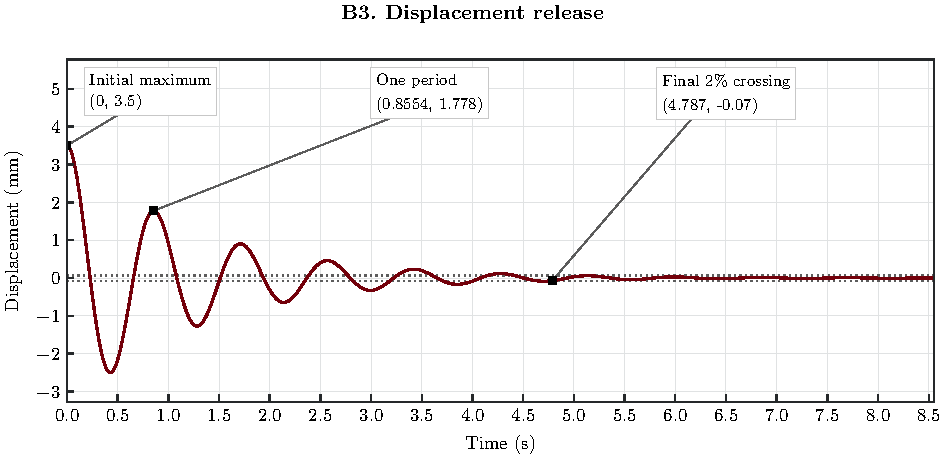
\includegraphics[width=0.95\linewidth,height=\textheight,keepaspectratio,alt={B.3. Exact final crossing and the 2 percent band. The plot shows ten damped oscillations and markers for the requested values.}]{figures/generated/solutions/B3.pdf}
\caption{B.3.11.a-b. Ten-cycle response with the initial maximum, one-period response, and final 2\% crossing.}
\end{figure}

\begin{figure}[H]
\centering
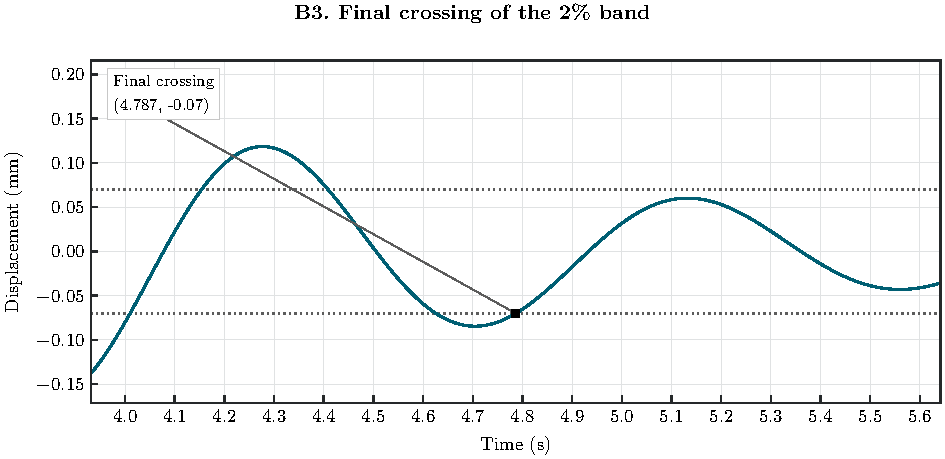
\includegraphics[width=0.95\linewidth,height=\textheight,keepaspectratio,alt={B.3. Detail of the final 2 percent crossing.}]{figures/generated/solutions/B3_settling.pdf}
\caption{B.3.11.c. Detail of the final 2\% crossing of the settling band.}
\end{figure}

\clearpage
\matlabcaption{MATLAB code used to reproduce the B.3.11 response plot.}

\lstinputlisting[style=hwmatlab]{matlab/B3.m}

The plot shows an underdamped response whose oscillation frequency remains constant while its amplitude decreases exponentially. The initial condition produces the largest displacement at release, and the displacement after one period is smaller by the factor $e^{-\zeta\omega_n\tau_d}$. The response first enters the 2\% band before $4.79\ \mathrm{s}$, but it does not remain there until the final crossing at $t_s=4.79\ \mathrm{s}$. The exponential envelope gives the conservative bound $t_{\mathrm{envelope}}=4.95\ \mathrm{s}$, which is later because the response is not at the envelope maximum at the exact crossing.

\text{(B.3.12)}
\endgroup
